\documentclass[runningheads,a4paper]{llncs}

\usepackage[latin1]{inputenc}
\usepackage{graphicx,color,url}
\usepackage[dvips]{epsfig}
\usepackage{verbatim}
\usepackage{tikz}
\usetikzlibrary{shapes,arrows}
\usetikzlibrary{calc,patterns,snakes,decorations.pathmorphing,decorations.markings}
\usetikzlibrary{positioning}

\newcommand{\keywords}[1]{\par\addvspace\baselineskip
\noindent\keywordname\enspace\ignorespaces#1}

\providecommand{\tabularnewline}{\\}

\begin{document}

\mainmatter  % start of an individual contribution

% first the title is needed
\title{Fuzzy Controller for TORCS}
% Antonio - T�tulo provisional, actualizar con el definitivo


% a short form should be given in case it is too long for the running head
\titlerunning{There can be only one}

% the name(s) of the author(s) follow(s) next
%
% NB: Chinese authors should write their first names(s) in front of
% their surnames. This ensures that the names appear correctly in
% the running heads and the author index.
%

%\author{M. Salem \and A.M Mora \and \and J. J. Merelo \inst{1}}
\author{A. N. Onymous\inst{1}%
\thanks{No Institute}}
% Antonio - Los autores que participen
%
\authorrunning{Anonymous, A}
% (feature abused for this document to repeat the title also on left hand pages)

% the affiliations are given next; don't give your e-mail address
% unless you accept that it will be published
%\institute{Dept. of Computer Architecture and Technology, University of Granada, Spain}
\institute{Anonymous Institute}


%
% NB: a more complex sample for affiliations and the mapping to the
% corresponding authors can be found in the file "llncs.dem"
% (search for the string "\mainmatter" where a contribution starts).
% "llncs.dem" accompanies the document class "llncs.cls".
%

\maketitle

%
%%%%%%%%%%%%%%%%%%%%%%%%%%%%%%%   ABSTRACT   %%%%%%%%%%%%%%%%%%%%%%%%%%%%%%%
%
\begin{abstract}
This paper is dedicated to design a fuzzy driver for racing car simulator. The proposed driver uses two fuzzy controller to obtain the steer and the target speed of the car using track borders sensors as inputs.\\
The  fuzzy controller is evaluated in practice and time trial races giving good results
%
%\keywords{Videogames, Fuzzy Controller, TORCS}

% Antonio - TODO: escribir mucho m�s completo
\end{abstract}

%
%%%%%%%%%%%%%%%%%%%%%%%%%%%%%%%   INTRODUCTION   %%%%%%%%%%%%%%%%%%%%%%%%%%%%%%%
%
\section{Introduction}
\label{sec:intro}
The Open Racing Car Simulator (TORCS) is one of the most popular car racing simulators among the scientific community. It was created by \textit{Eric Espi�} and \textit{Christophe Guionneau}, and due to its open-source philosophy, there are several designers and programmers constantly improving it \cite{manualTORCS}.
TORCS \cite{WebTORCS} is a three-dimensional racing video game, mainly aimed to serve as a framework to develop and test Artificial Intelligence (AI) models for autonomous drivers, named \textit{controllers} or \textit{bots}.

Even if it has not the graphic quality of commercial games, it presents several advantages for academic purposes, such as \cite{manualTORCS}:

\begin{itemize}
	\item  It lies between an advanced simulator, like recent commercial
	car racing games, and a fully customisable environment,
	like the ones typically used by computational
	intelligence researchers for benchmark purposes.
	\item  It features a sophisticated physics engine (aerodynamics,
	fuel consumption, traction) as well as a 3D graphics
	engine for the visualisation of the races.
	\item  It was not conceived as a free alternative to commercial
	racing games, but it was specifically devised to make it
	as easy as possible to develop and test your own controller. 
   In fact, controllers are implemented as separated software pieces with 		 
   modular architecture, so it is easy to develop a new one and to plug 
	it into the game.
\end{itemize}

Even in simulation mode, driving a car with a bot as a human would do is a hard task, because the agent has to control several actions such as the steer, gear and brake/acceleration using the data related to the car and its environment (detected by means of sensors).

Fuzzy logic \cite{abraham2001} with its adaptation and ability of imitating the human behaviour, is an interesting tool to design automatic TORCS drivers. It could be integrated in any controller module (steer, gear, acceleration and brake, stuck) to give a human-like `appeal' to the bot driver \cite{CarRacing_Pelta09,Guadarrama2008}. 

In each simulation tick, the autonomous driver must make a decision, for instance, to direct the car (steer) on the track and select a target speed. This problem is much harder when the car is near to a curve where it has to choose a compromise between going faster and avoiding the car slips and goes out of the track. The overall idea is to move the car towards the farthest track border to avoid prematurely breaking.

This complex problem could be solved by means of fuzzy logic, due to its adaptive control and dealing with noise and uncertainty. 
% Antonio - Aclarar qu� es ruido o qu� tipo de ruido hay en el problema. Igual con la incertidumbre. ;)
Indeed, many researchers have taken advantage of this technique to design TORCS controllers: \cite{Guadarrama2008,neurone,CarRacing_Pelta09}. In the latter, for instance, a fuzzy controller was designed to obtain the target position and the steer was computed through a crisp formula. 
% Antonio - �y en los dos trabajos anteriores qu� se hace? Hay que destacar las diferencias de este estudio con respecto a todos los que hay en la literatura del mismo tipo (controladores fuzzy). Para as� destacar por qu� se ha hecho este y por qu� es mejor y avanza el estado del arte. ;)
% Salem - 
% Antonio - contar algo m�s del problema y justificar la necesidad de este trabajo respecto a lo que hay hasta ahora (motivation). �Por qu� usar Fuzzy Logic es una mejor idea que a las otras que hay? 
% As� como lo que aportar� al estado del arte y c�mo lo har� avanzar (contribution). �No hay nada parecido?�Abre una nueva l�nea de investigaci�n?
% Como s� hay otros trabajos que aplican FL para crear controladores, hay que diferenciar este de los otros y justificar por qu� este es mejor. ;)
% Aqu� se hace un peque�o resumen de esto y en el estado del arte se hace una comparativa m�s profunda respecto a los trabajos existentes.

However, in this work we present a novel fuzzy-based controller, which computes the steer and target speed using two specialised fuzzy sub-controllers.
They consider the track sensors (to find the farthest border) and the opponents' position in the race (for collision avoidance and overtaking).
% Salem - 
% Antonio - comentar un poco (entre par�ntesis, por ejemplo) los sensores de la pista considerados. �No se usan sensores del coche?�Por qu�?

The remainder of this paper is organised as follows:
The next section presents the state of the art and related works, and comments their differences with regard to this study, along with its contribution to advance in this research line. TORCS simulator is described in Section \ref{sec:torcs}.
The proposed fuzzy controller (and its sub-controllers) is detailed in Section \ref{sec:fuzzy_controller}, whereas it is tested in `real' (simulated) races in Section \ref{sec:results}. Obtained results are analysed and compared 
with other controllers are given in the same section. Finally, the conclusions and future lines of work are included in Section \ref{sec:conclusions}.


%%%%%%%%%%%%%%%%%%%%%%%%%%%%%%  STATE OF THE ART  %%%%%%%%%%%%%%%%%%%%%%%%%%%%%
%
\section{Background and State of the Art}
\label{sec:soa}

% Antonio - TODO: by Antonio and Fergu (Work in progess)



%%%%%%%%%%%%%%%%%%%%%%%%%%%%%%  TORCS 
In the last years, several researchers have focused on driving a racing car using computational intelligence techniques \cite{evol},\cite{torcs2012}, \cite{neurone}  and especially fuzzy logic where \cite{CarRacing_Pelta09} tried to design a fuzzy controller for the the target speed while the other car actions were obtained by simple functions while in\cite{ho2008}, a  previous fuzzy controller was enhanced using context-dependent fuzzy set, the obtained controller was compared to existing driving 
techniques showing better performance.\\
In \cite{Guadarrama2008}, a fuzzy rule-based car controller for Car Racing Competition was built and tuned with coevolutionary genetic algorithms. Its results had been compared with  cooperative and competitive approaches to tuning parameters.
Authors of \cite{Fujii2008} had examined the performance of fuzzy rule-based systems in  high-level decision making of a car and the effect of sensory information. 
 %%%%%%%%%%%%%%%%%%%%%%%%%%%%%
%
\section{Problem Description: TORCS}
\label{sec:torcs}

The Open Racing Car Simulator (TORCS)\cite{WebTORCS} is a standalone application mainly designed as a framework or testbed for bots/controllers, which are built as separate modules loaded into the main memory when a race takes place \cite{Torcs3}, so they are quite independent fro the game engine itself.
The main features of the architecture of TORCS are \cite{manualTORCS}: 

\begin{itemize}
	\item TORCS is a client-server application, where the bots are run as external processes connected to the server through UDP connections.
	\item The simulation is achieved in real time with 20 ms per game tick. So, the server sends the values of the sensors to every controller and waits 10 ms (real time) to receive an action to conduct from the bot.
	If there is not a new action, the simulation continues and the last action is repeated.
	\item The TORCS software makes a physical separation between the driver code and the simulator itself. Hence, it defines an abstract layer that gives complete freedom of choice of the programming language used to implement the bots, and just gives access to some information.
\end{itemize}

There are several competitions which use TORCS as base. During a competition, the bot perceives the race environment by means of a number of sensors, that provide information such as the status of the car, the status of the race, opponents positions and track borders \cite{manualTORCS,torcs2}.
Table \ref{t1} presents a complete list of available sensors with a description of each one.

\begin{table}[h!]
	
	\begin{tabular}{|p{2cm}|p{3cm}|p{3 cm}|p{4 cm}|}
		\hline
		{\textbf{Sensor} }&
		{\textbf{Name} }&
		{\textbf{Range} (unit)} &  
		{\textbf{Data type}}\\ 
		\hline
		1 & angle & [-$\pi$,+$\pi$ ] & Double\\ 
		\hline
		2 & curLapTime & [0,+$\infty$] (s)	& Double\\ 
		\hline 
		3 & damage & [0,+$\infty$)(point)& Double\\ 
		\hline 
		4 & distFromStart & [0,+$\infty$) (m)& Double \\ 
		\hline 
		5 & distRaced &[0,+$\infty$) (m)& Double\\
		\hline 
		
		6 & focus & [0,200] (m)& Double\\
		\hline 
		
		7 & fuel & [0,+$\infty$) (l)& Double\\
		
		\hline
		8 & gear & \{-1,0,1,.. 6\}g& Integer \\
		
		\hline
		9 & lastLapTime &[0,+1] (s) & Double \\
		
		\hline
		10 & opponents &[0,200] (m)& Double \\
		
		\hline
		10 & racePos & \{1,2,...,N\} & Double \\
		\hline
		11 & rpm    & [0,+$\infty$) (rpm)   & Double \\
		\hline  
		13 & speedX & (-$\infty$,+$\infty$) (km/h) & Double\\
		\hline  
		14 & speedY &(-$\infty$,+$\infty$) (km/h)  & Double\\
		\hline 
		15 & speedZ & (-$\infty$,+$\infty$) (km/h) & Double \\
		
		\hline
		16 & track &  [0,200 ] & Double\\ 
		\hline
		17 & trackPos & (-$\infty$,+$\infty$) & Double\\
		
		\hline
		
		18 & wheelSpinVel  & [0,+$\infty$) (rad/s) & Double\\
		
		\hline
		19 & z &  (-$\infty$,+$\infty$) (m) & Double\\
		
		\hline
		
	\end{tabular}
	\caption{Description of available sensors in TORCS \cite{Torcs3}.}
	\label{t1}
\end{table}

Every TORCS driver bot is controlled by means of a set of actuators: the steering wheel 'Steer', the accelerator 'accel', the brake pedal and the gearbox. In addition, a meta-action is available to request a restart of the race to the server. Table \ref{tab2} details the available actions/actuators and their representation.

\begin{table}[t!]
	
	\begin{tabular}{|p{3cm}|p{3 cm}|p{6 cm}|}
		\hline
		
		{\textbf{Action} }&
		{\textbf{Range} (unit)} &  
		{\textbf{Data type}}\\ 
		\hline
		Acceleration & [0,+1] & Double\\ 
		\hline
		Brake & [0,+1]	& Double\\
		\hline
		Gear & -1..0..+6	& Double\\
		\hline
		Steer & [-1,+1]	& Double\\
		\hline
		Clutch & [-1,+1]	& Double\\
		\hline
	\end{tabular}
	\caption{TORCS Actuators \cite{torcs}}
	\label{tab2}
\end{table}

Hence, a controller is a program, which run inside TORCS, that automatically drives a car. It gets as input information about the current state of the car and its situation on the track. These collected data are used to compute actions to do in the next simulation tick; like steer, gear changes, acceleration or brake and clutch. A client may request a restart of the race by sending a special action on the server: Restart or shutdown \cite{manualTORCS}.

The basic architecture of a controller consists of five simple modules (see Figure \ref{archi}). 
% This modular architecture is a key factor to achieve good results.
% Antonio - �por qu�?

\begin{figure}
	
	\centering
	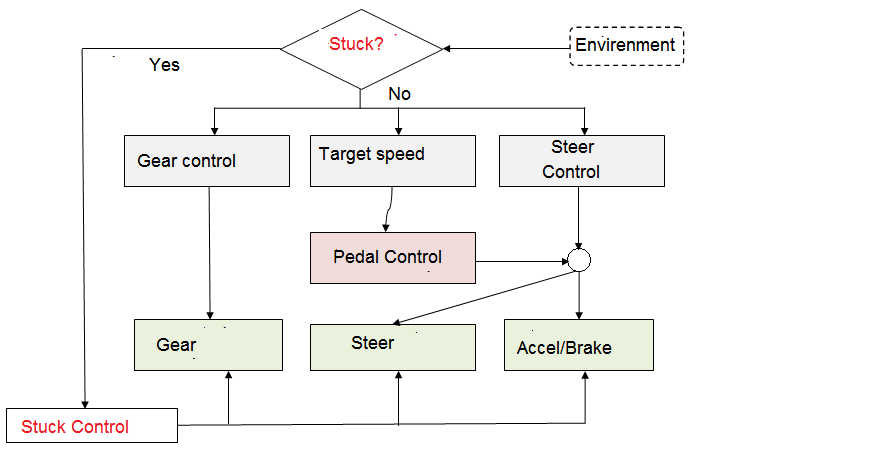
\includegraphics[width=0.9\textwidth]{fig/archicontrole2.PNG}
	\begin{minipage}{10cm}
		\centering
		\caption{\footnotesize Controller's Architecture.}
		\label{archi}
	\end{minipage} 	
\end{figure}
	
TORCS comes with a simple example driver often used to validate new designed controllers \cite{torcs,torcs2}. 
%It presents very basic functions for controlling the race car to give developers an idea of what the controller should look like. It includes simple functions to control the speed, steering angle and speed without dealing with opponents. 
% Antonio - lo quito para ahorrar espacio



%%%%%%%%%%%%%%%%%%%%%%%%%%%  FUZZY CONTROLLER  %%%%%%%%%%%%%%%%%%%%%%%%%%%%
%
\section{Proposed Fuzzy Controller}
\label{sec:fuzzy_controller}

The proposed controller has the same modular architecture as the simple driver where the target speed  and steer values are  computed via fuzzy controller using five position sensors.

\subsection{Fuzzy target speed}
To estimate the target speed  based on fuzzy rules, two cases are considered.
\begin{enumerate}
	\item If the car is in straight line, the target speed will take a maximum value (maxSpeed).\\
	\item If it is near a curve, the controller will decrease its current speed to a value included in the interval [minSpeed; maxSpeed] km/h.
\end{enumerate}
In case the car is off the track or near a curve, the brake system is activated where  the ABS and TCS will be loaded to avoid the car skidding.
\\
The obtained target speed will be used in calculating the value of acceleration.
\begin{equation}	
Gas(speed-Target_{speed})=-1+\frac{2}{1+e^{speed-Target_{speed}}}	
\end{equation}

Gas is for acceleration, Speed is the  current speed of the car.\\
Our fuzzy controller has 3 input values and one output: the target speed value(See figure \ref{AD}):

\begin{figure}
	\begin{center}
		
		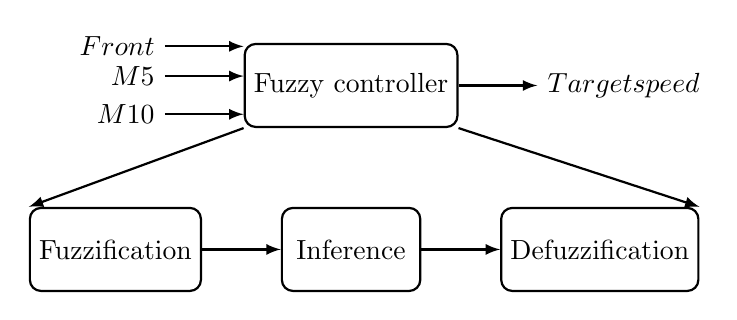
\begin{tikzpicture}[box/.style={draw, fill=white!20,rounded corners,align=center,minimum height=3em, minimum width=5em},thick,->,>= latex]
		
		\node[box] (a0) {Fuzzy controller};
		\node[left=of a0.160,font=\bfseries] (aux01) {$Front$};
		\node[left=of a0.175,font=\bfseries] (aux02) {$M5$};
		\node[left=of a0.195,font=\bfseries] (aux03) {$M10 $};
		\node[right=of a0,font=\bfseries] (c0) {$Target speed$};
		\draw[thick,->,>= latex] (aux01) -- (a0.160);
		\draw[thick,->,>= latex] (aux02) -- (a0.175);
		\draw[thick,->,>= latex] (aux03) -- (a0.195);
		\draw[thick,->,>= latex] (a0) -- (c0);
		\node[box,below=of a0] (b) {Inference};
		
		\node[box, left=of b] (a) {Fuzzification};

		
		\node[box,right=of b] (b1) {Defuzzification};

	
		\draw[thick,->,>= latex] (a) -- (b);
		\draw[thick,->,>= latex] (b) -- (b1);
	
		
		
		\draw[thick,->,>= latex] (a0.south west) -- (a.north west);
		\draw[thick,->,>= latex] (a0.south east) -- (b1.north east);
		
		
		\end{tikzpicture}
		
		%\includegraphics [width=10cm,height=4cm]{figures/c2/sif}
	\end{center}
	\caption{Fuzzy control of target speed.}     % width is 8.4 cm.
	\label{AD}
\end{figure}

The fuzzy driver (FD) is a Mamdani based fuzzy system \cite{Iancu2012} (See fig.\ref{AD}) with trapezoidal membership functions for input variables. It uses three values among the 19 of the track sensor (See fig.\ref{fig34}):

\begin{enumerate}
	\item Front = Track[9]  with angle = 0 , the front distance between the car and the border of track.
	\item M5 = max (Track[8]; Track[10])
	the max distance with +5 and  -5 angle.
	\item M10 = max (track[11]; track[7]) ,	the max distance with +10 and  -10 angle.
\end{enumerate}
\begin{figure}[h!]
	
	\centering
	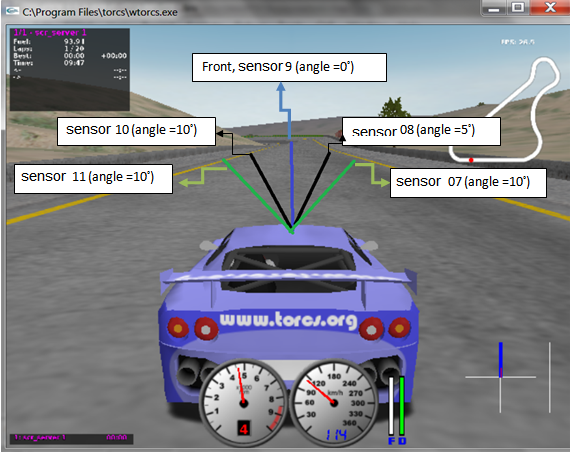
\includegraphics[width=0.9\textwidth]{fig/sensor22.png}
	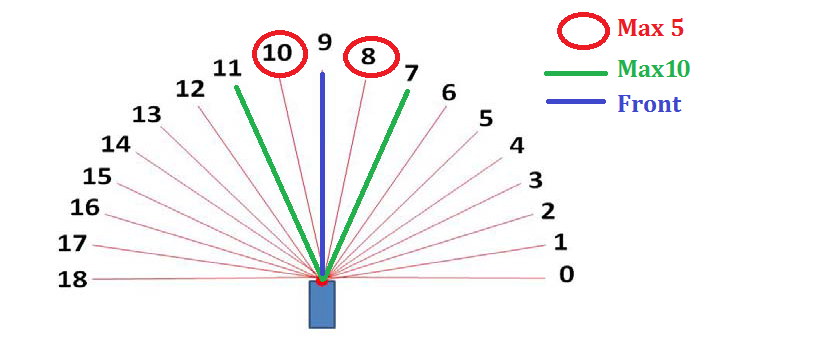
\includegraphics[width=0.9\textwidth]{fig/front.png}
	\begin{minipage}{10cm}
		\centering
		\caption{\footnotesize Fuzzy inputs.}
		\label{fig34}
	\end{minipage} 		
\end{figure}
Each input variable is represented by three membership functions Low, Medium and High\\
The description of fuzzy inputs and output are represented in table \ref{flouevar} .
	
	\begin{table}
		\label{flouevar}
		\caption{ Fuzzy variables description}
		\begin{tabular}{ |p{1cm}|p{2cm}|p{1.5cm}|p{2 cm}|p{1 cm}|p{1.5 cm}|p{1.5 cm}|}
			\hline
			{ \color{red} Variable }&
			{ \color{red}Range }&
			{ \color{red}Name}&  
			{ \color{red} MF } &
			{ \color{red} Low } &
			{ \color{red} Medium }&
			{ \color{red} High } 
			
			\\
			\hline
			Input & [0-100] m & Front & trapezoidal & [0-50] & [20-80] &[80-100]
			\\
			\hline
			Input & [0-100] m & M5 & trapezoidal &[0-40] & [10-70] & [40-100] 
			\\
			\hline
			Input & [0-100] m  & M10 & trapezoidal & [0-30] & [0-60] & [30-100]
			\\
			\hline 
			Output & [0-200]m/s & TS & singleton & / & / & /
			\\
			\hline 
		\end{tabular} 
	\end{table}

	The rules base is designed so that if the front distance is maximal, then target speed should be maximal, and this value should be less when  the frontal distance is lower. The fuzzy rules are listed below:
	\\
	\begin{enumerate}
		\item If Front is High Then TargetSpeed is TS1
		\item If Front is Medium Then TargetSpeed is TS2
		\item If Front is Low and M5 is High Then TargetSpeed is TS3
		\item If Front is Low and M5 is Medium Then TargetSpeed is TS4
		\item If Front is Low and M5 is Low and M10 is High Then TargetSpeed is TS5
		\item If Front is Low and M5 is Low and M10 is Medium Then TargetSpeed is TS6
		\item  If Front is Low and M5 is Low and M10 is Low Then TargetSpeed is TS7
		\\
		In addition, a crisp rule is added to rule base to obtain a maximum value of the target speed when the three input variables are as big as possible: \\
		\item If Front = Maxdistspeed or M5 = Maxdistspeed or M10 = Maxdistspeed Then TargetSpeed = Maxspeed	
		
	\end{enumerate}
	The output value (target speed) is encoded by seven singletons.
	
	\subsection{Fuzzy Steer control}	
	We can use another fuzzy controller to control the Steer to estimate and determine the target position of the car:\\
	if the car is straight line then it will take as target position half width of the race track.	
	
	If the car is near a right curve,it will approach the path leading to the right, with a space between the car and the border of the track to avoid the loss of control and shocks .The same if the car is near a left curve. \\
	
	Detection of curves is based on the sensor values (M10, M5, front).
	the rule base is presented as follows:\\
	\begin{itemize}
		
		\item If Front is High Then steer is S1
		\item If Front is Medium Then steer is S2
		\item If Front is Low and M5 is High Then steer is S3
		\item If Front is Low and M5 is Medium Then steer is S4
		\item If Front is Low and M5 is Low and M10 is High Then steer is S5
		\item If Front is Low and M5 is Low and M10 is Medium Then steer is S6
		\item  If Front is Low and M5 is Low and M10 is Low Then steer is S7
		\\
	\end{itemize}	

%%%%%%%%%%%%%%%%%%%%%%%%%%%%%%  RESULTS  %%%%%%%%%%%%%%%%%%%%%%%%%%%%%
%
\section{Simulation Results}
\label{sec:results}

In this section we present all the experiments that we performed in order to measure the performance of our "FD" controller .
We first, describe the methodology we have used and next, we present the experimental results of the implementation of the Fuzzy driver, with opponents and
using special criteria in each case. \\
We have established a set of tests to measure the performance of the controller "AD". We compared the newly developed Controller with existing methods: the simple driver. We will run every controller in several race tracks. 
\subsection{Simulation settings}
TORCS provides different tracks to choose from. These race tracks are designed by different developers in order to test the performance of the controllers on different difficulty circuits and on different types of roads.\\

In our case, we chose three of road tracks, a dirt road, and an oval track.\\


On oval tracks, E-Track5 seems to be the most interesting, as it has curves in both directions. On dirt roads, Dirt1 has a good variety of curves. For road tracks, we selected three tracks: Forza, E-Road and CG-Speedway Number1. Table \ref{Tabtrack}  presents the properties and description of each selected track.\\

\begin{table}
	
	\caption{Description of Selected tracks}
	\label{Tabtrack}
	\begin{tabular}{ |p{2cm}|p{2 cm}|p{2 cm}|p{2 cm}|p{2 cm}|p{2 cm}|}
		\hline
		\textbf{Track name}    & E-Track5
		& Dir1 4 
		& Forza
		& E-Road
		& CG-Speedway Number1
		\\
		\hline
		\textbf{Shape}   
		& 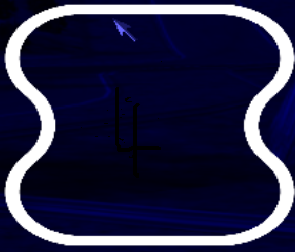
\includegraphics[scale=0.3]{fig/track4.png}
		& 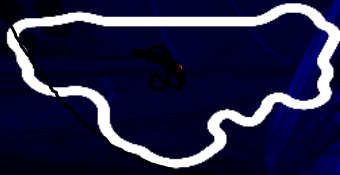
\includegraphics[scale=0.3]{fig/track2.png}
		& 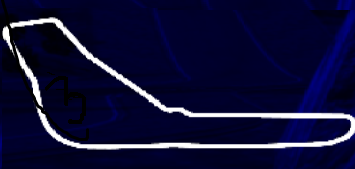
\includegraphics[scale=0.3]{fig/track3.png}
		&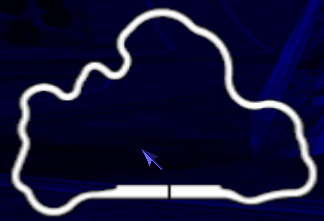
\includegraphics[scale=0.3]{fig/track5.png}
		& 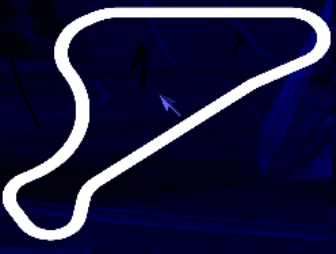
\includegraphics[scale=0.3]{fig/track1.png}
		
		\\
		\hline
		\textbf{Track Type}   
		& Oval
		& Dirty
		& Road
		& Road
		& Road
		
		\\
		\hline
		
		\textbf{Length}   
		& 1621.73 m
		& 3260.43 m
		& 5784.10 m
		& 3260.43 m
		& 2057.56 m
		
		\\
		\hline
		\textbf{Width}   
		& 20.0 m
		& 16.0 m
		& 11.0 m
		& 16.0 m
		& 15.0 m
		\\
		\hline
	\end{tabular} 
\end{table}
\subsubsection{ Cars settings}

SCR 1 server is a NASCAR car and member of the SCR Server team (A team can used different types of car as  car1-stock1, car1-tbr1 ...).\\
A Sprint Cup Series NASCAR-type car weighs at least 1542 kg for 850 horses with . The engine is a V8 with  $ 5,866 cm ^ 3 $. Its chassis is tubular type. It has a Borg-Warner gearbox with four-speed for road circuits.\\

In our simulations, we used the car "car1-tbr1" which has a weight of 1150 KG, max fuel: 94 KG, length= 4.25 m and a width of 1.94 m.
\subsubsection{Controllers settings}
To validate the fuzzy controllers, we have considered the following controllers:\\
AD1: Fuzzy target speed  controller \\
AD2: Fuzzy steer and speed controller \\
AD5: Fuzzy target speed  controller with opponent consideration \\
SD: Simple driver \\

We conducted a series of experiments to measure the performance of the best version control in some race tracks (05 tracks in table \ref{Tabtrack} ).

\subsection{Results of 20 lap practice race}
In this case, we tested our controllers in a 20 laps practice race in the four tracks:\\
	
In this section, we set the distance to 20 laps for each track and for each controller. 
\begin{table}  
	
	\caption{Results for 20 laps}
	\label{resultat1}

	\begin{tabular}{ |p{3cm}|p{2cm}|p{2cm}|p{2 cm}|p{2 cm}|}
		
	\multicolumn{5}{c}{\textbf{E-Track5}}\\
		\hline
		{ \color{blue}\textbf{20 laps} }&
		{ \color{red}\textbf{SD}}&  
		{ \color{red} \textbf{AD1} } &
		{ \color{red} \textbf{AD2} } &
		{ \color{red} \textbf{AD5} }
		\\
		\hline
		Best Time & 01:05:15  & 01:21:24  &04:33:24 & 29:87 
		\\
		\hline
		Topspeed & 149  & 148 & 203 & 199 
		\\
		\hline
		Minspeed & 46 & 44 & 60 & 172 
		\\
		\hline 
		Lastlap	Time  & 01:05:17 & 01:31:36 & 01:02:55 & 30:07
		\\
		\hline 
		Best lap & 14 & 02 & 18 & 8 
		\\
		\hline
		Damage & 0 & 0 & 0 & 0 
		\\
		\hline 
		Fuel & 71:22 & 71:25 & 77:45 & 77:02 
		\\
		\hline
\multicolumn{5}{c}{\textbf{Dirt}}\\	
		\hline
		{ \color{blue}\textbf{20 laps} }&
		{ \color{red}\textbf{SD}}&  
		{ \color{red} \textbf{AD1} } &
		{ \color{red} \textbf{AD2} } &
		{ \color{red} \textbf{AD5} }
		\\
		\hline
		Best Time & 01:12:96 & 50:43  &02:23:12  & 35:51 \\
		\hline
		Topspeed & 132  & 126 & 136 & 139 
		\\
		\hline
		Minspeed &  21 & -52 & -43 & -54 
		\\
		\hline 
		
		
		Lastlap	Time  & 01:13:08  & 02:33:43 & 02:23:12 & 01:02:91 
		\\
		\hline 
		Best lap & 14 & 07 & 01 & 5 
		\\
		\hline
		Damage &  0 & 7438 & 905 & 9274 
		\\
		\hline 
		Fuel & 65:04 & 79:26 & 79:98 & 66:06 
		\\
		\hline
\multicolumn{5}{c}{\textbf{Forza}}\\	
		\hline
		{ \color{blue}\textbf{20 laps} }&
		{ \color{red}\textbf{SD}}&  
		{ \color{red} \textbf{AD1} } &
		{ \color{red} \textbf{AD2} } &
		{ \color{red} \textbf{AD5} }
		\\
		\hline
		Best Time & 03:03:66  & 02:39:82 & 07:14:90  & 02:20:27 
		\\
		\hline
		Topspeed & 149 & 248 & 209 & 246 
		\\
		\hline
		Minspeed & 22  & -41 & -53 & 63 
		\\
		\hline 	
		Lastlap	Time  & 03:03:66 & 02:47:26 & 09:55:62 & 02:21:23
		\\
		\hline 
		Best lap & 20 & 04 & 01 & 04 
		\\
		\hline
		Damage & 0 & 468 & 2269 & 0 
		\\
		\hline 
		Fuel & 62:61 & 71:88 & 60:55 & 60:55
		\\
		\hline
	\multicolumn{5}{c}{\textbf{E-Road}}\\	
		\hline
		\hline
		{ \color{blue}\textbf{20 laps} }&
		{ \color{red}\textbf{SD}}&  
		{ \color{red} \textbf{AD1} } &
		{ \color{red} \textbf{AD2} } &
		{ \color{red} \textbf{AD5} }
		\\
		\hline
		Best Time & 02:44:93  & 02:11:39 & 04:33:59 & 01:25:66 
		\\
		\hline
		Topspeed & 149  & 202 & 203 & 207 
		\\
		\hline
		Minspeed & 24  & -58 & 32& -55 
		\\
		\hline 
		
		Lastlap	Time  & 02:45:08 & 03:00:20 & 04:51:53 & 01:27:38 
		\\
		\hline 
		Best lap & 3 & 3 & 17 & 03
		\\
		\hline
		Damage & 0 & 6056 & 7309 & 2239 
		\\
		\hline 
		Fuel & 62:11 & 78:25 & 79:25 &  55:22 
		\\
		\hline
\multicolumn{5}{c}{\textbf{CG-Speedway Number1}}\\	
		{ \color{blue}\textbf{20 laps} }&
		{ \color{red}\textbf{SD}}&  
		{ \color{red} \textbf{AD1} } &
		{ \color{red} \textbf{AD2} } &
		{ \color{red} \textbf{AD5} }
		\\
		\hline
		Best Time & 01:25:00  & 01:12:99 & 01:12:23& 53:61 
		\\
		\hline
		Topspeed & 149  & 191& 194 & 178 
		\\
		\hline
		Minspeed & 49 & 57 & 32 & -51 
		\\
		\hline 
		
		Lastlap	Time  & 01:25:01 & 01:12:99& 01:29:65 & 01:46:47 
		\\
		\hline 
		Best lap & 12 & 20 & 02 & 02  
		\\
		\hline
		Damage & 0 & 0 & 0 &  114 
		\\
		\hline 
		Fuel & 66:66 & 62:58 & 73:38 & 60:65 
		\\
		\hline
	\end{tabular} 
	\label{Result1r}
\end{table}

The table \ref{Result1r} shows that among the four drivers, the minimum time has been reached by the AD5 controller in each of the five tracks, this was due to the steering unit of the target. The target position allows the car to adjust safely the required steering angle  with the maximum speed so the controller AD5 gave the best time.
\\
However, taking a smaller target angle required a greater distance to cover by car by taking a less efficient trajectory. In addition, the number of times the car was off the road on Dir1 and Forza was higher for AD5 and, accordingly, the time that the car has passed out of the track was potentially higher than the other controllers.\\	
Thus, higher damages happened after the collision with the outer walls of the track when the car is off the track. The simple SD driver finished the race without damage, while AD5 was able to complete all the tracks safely except the Dir1t4 and Forza circuit where the damage is a little high for the AD1 driver (fig.\ref{resultat1}). For the fuel consumption, it  depends on  shocks rate and category of tracks.

\subsection{Time trial race}
Now, we set the race stopping criterion to 300s, so each controller is run in a time trial race where the race is stopped after 300s and the current distances are compared.
Results are in Table \ref{resulta9}.
\begin{table} 
	
	\caption{Results of the controllers in 5 minute time trial race}
	\label{resulta9}
	\begin{tabular}{ ||p{3cm}||p{3cm}||p{3cm}||p{3 cm}||}	
		\multicolumn{4}{c}{\textbf{E-Track5}}\\	
		
		\hline
		{ \color{blue}\textbf{} }&
		{ \color{red}\textbf{Best Time} }&
		{ \color{red} \textbf{Distance } } &
		{ \color{red} \textbf{Top speed} }
		\\
		\hline
		AD1 &01:11:98  &4540,844&  155
		\\
		\hline
		AD2 & 02:15:26 &8803,161& 155
		\\
		\hline 
		AD5 & 29:30&32600&199 
		\\
		\hline 
		\multicolumn{4}{c}{\textbf{Dir1}}\\			
		\hline
		{ \color{blue}\textbf{} }&
		{ \color{red}\textbf{Best Time} }&
		{ \color{red} \textbf{Distance } } &
		{ \color{red} \textbf{Top speed} }
		\\
		\hline
		AD1 & 52:27 & 7825,032&126  
		\\
		\hline
		AD2 & 00:00 &5202,99& 134
		\\
		\hline 
		AD5 & 00:00 &620,25& 153 
		\\
		\hline 
		\multicolumn{4}{c}{\textbf{Froza}}\\		\hline
		{ \color{blue}\textbf{} }&
		{ \color{red}\textbf{Best Time} }&
		{ \color{red} \textbf{Distance(m) } } &
		{ \color{red} \textbf{Top speed(m/s)} }
		\\
		\hline
		AD1 & 02:49:12  &17352,3  &  247
		\\
		\hline
		AD2 & 02:49:12  & 17354,12 & 239
		\\
		\hline 
		AD5 & 57:66 & 17355,2 & 203 
		\\
		\hline 
	\multicolumn{4}{c}{\textbf{E-Road}}\\	
		\hline
		{ \color{blue}\textbf{} }&
		{ \color{red}\textbf{Best Time} }&
		{ \color{red} \textbf{Distance } } &
		{ \color{red} \textbf{Top speed} }
		\\
		\hline
		AD1 & 03:62:33 & 11586,2 &  160
		\\
		\hline
		AD2 & 02:41:41  & 11588 & 208 
		\\
		\hline 
		AD5 & 01:15:16 & 23139 & 217
		\\
		\hline 
			\multicolumn{4}{c}{\textbf{CG-Speedway Number1}}\\
		\hline
		{ \color{blue}\textbf{} }&
		{ \color{red}\textbf{Best Time} }&
		{ \color{red} \textbf{Distance } } &
		{ \color{red} \textbf{Top speed} }
		\\
		\hline
		AD1 & 01:15:19 & 23136 &  195
		\\
		\hline
		AD2 & 01:15:80 & 17352,2 & 193 
		\\
		\hline 
		AD5 & 44:67& 28921,6 &206 
		\\
		\hline 
		
	\end{tabular}
\end{table}
\subsection{Real race}
Our main goal is to test the performance of "AD5" in a race, and answer the following questions: Could we have a perfect driving in a race with "AD5" only with the track borders sensors? Can we win the race with AD5?\\
In this context we tested "AD5" in 5 tracks against berwin,bt, damned, inferno and tita teams.\\
After the launch of the race "AD5" against the 10 cars of each team  for 20 laps in each track we obtained the following results (see table \ref{resultat31})
\begin{table}
	\caption{Results of AD5  in a real race}
	\label{resultat31}
	\begin{tabular}{ |p{3cm}|p{2cm}|p{2cm}|p{2 cm}|p{2 cm}|p{2 cm}|}
		\hline
		{ \color{blue}\textbf{E-Track5} }&
		{ \color{red}\textbf{Against berwin team }}&  
		{ \color{red} \textbf{Against bt team} } &
		{ \color{red} \textbf{Against damned team} } &
		{ \color{red} \textbf{Against inferno team} }&
		{ \color{red} \textbf{Against tita team} }
		\\
		\hline
		Ranking & 1/11 & 2/11   & 1/11 & 7/11& 4/11
		\\
		\hline
		race time & 02:36:78 & 02:40:38+ 03:41   & 02:42:73 & 02:15:81 + lap & 02:18:74 + 28:19
		\\
		\hline
		Best time & 29:90 & 30:28   & 30:28 & 30:59& 30:53 
		\\
		\hline 
		Maxspeed & 198 & 198 &  198 & 199 & 198
		\\
		\hline
		
		Damage & 2267 & 7939 &  5888 & 5232& 8043
		\\
		\hline 
		
		
		Pit stops & 0& 0  & 0 & 0 & 0
		\\

		\hline
		\hline
		{ \color{blue}\textbf{Froza} }&
		{ \color{red}\textbf{Against berwin team }}&  
		{ \color{red} \textbf{Against bt team} } &
		{ \color{red} \textbf{Against damned team} } &
		{ \color{red} \textbf{Against inferno team} }&
		{ \color{red} \textbf{Against tita team} }
		\\
		\hline
		Ranking & 10/11  & 11/11 & 11/11 & 10/11& 10/11
		\\
		\hline
		Race time & 7:44:99 + Lap & 8:07:39 + 02:16:32 & 08:09:42 + 1Lap & 6:40:33 + Lap 0 &  6:37:02 + Lap 
		\\
		\hline
		Best time & 01:57:58 & 01:45:30 & 02:03:00 & 02:04:00& 02:04:37
		\\
		\hline 
		Maxspeed & 243  & 282 & 260 & 220& 217
		\\
		\hline
		
		Damage & 2275 & 95 & 475 & 416 & 1185
		\\
		\hline 
		
		
		Pit stops & 0 & 0 & 0 & 0 & 0
		\\
		\hline	
	\end{tabular} 
	
\end{table}

From Table \ref {resultat31}, we noticed that our controller has won a race only in some types of tracks such as "E-track5" category "Oval track".\\

When our controller is in parallel with his opponent, and the distance between them is smaller, and they are in a smaller width track,  there is a possibility of  damage.
\\

According to damage results, despite our controller can win the race on the E-track5 but it had a higher crash rates in the majority of cases. We observed also that in the majority of cases our car is very slow compared to the other cars in each team. 
%%%%%%%%%%%%%%%%%%%%%%%%%%%%%  CONCLUSIONS  %%%%%%%%%%%%%%%%%%%%%%%%%%%%
%
\section{Conclusions and Future Work} 
\label{sec:conclusions}
 



%%%%%%%%%%%%%%%%%%%%%%%%%%%%%%%%%%%%%%%%%%%%%%%%%%%%%%%%%%%%%%%%%%%%%%%

\section*{Acknowledgments}

Omitted for Blind reviews.

%This work has been supported in part by projects 
%EPHEMECH (TIN2014-56494-C4-3-P, Spanish Ministerio de Econom�a y Competitividad), 
%PROY-PP2015-06 (Plan Propio 2015 UGR), 
%PETRA (SPIP2014-01437, funded by Direcci�n General de Tr�fico),
%CEI2015-MP-V17 (awarded by CEI BioTIC Granada), and 
%PRY142/14 (funded by Fundaci�n P�blica Andaluza Centro de Estudios Andaluces en la IX Convocatoria de Proyectos de Investigaci�n).


\bibliographystyle{splncs03}
\bibliography{fuzzy_torcs}



\end{document}
